% Compile with pdflatex (twice) or tectonic. Figures: slides/figures/*.pdf (copies of results/figures/report/).
% 10 main slides + 3 backup slides; about 10 minutes + 5 minutes viva/demo. Each student speaks for about 5 minutes.
\documentclass[aspectratio=169,11pt]{beamer}
\usetheme{Warsaw}
\usecolortheme{default}
\usepackage[T1]{fontenc}
\usepackage{lmodern,amsmath,booktabs,tabularx,graphicx}
\definecolor{afgml}{RGB}{22,57,86}
\setbeamercolor{structure}{fg=afgml}
\setbeamertemplate{navigation symbols}{}
\setbeamertemplate{footline}[frame number]
\newif\ifguidance\guidancefalse
\newcommand{\help}[1]{\ifguidance\begin{block}{Preparation guidance}\small #1\end{block}\fi}
\newcommand{\fillin}[1]{[\textit{#1}]}
\newcommand{\EO}{\Delta_{\mathrm{EOdds}}}
\title[AFGML Capstone]{Problem 5: Fairness Transfer across States and Years}
\subtitle{ICT 5143: AFGML Capstone}
\author{Aslam Mugutkhan, 261090830010 \and Rao Ashlesha Padmananda, 261090830019}
\date{07/11/26}
\begin{document}
% Slide 1: 20 seconds. Student 1 introduces team and question.
\begin{frame}\titlepage\end{frame}

% Slide 2: 50 seconds.
\begin{frame}{Research question and decision context}
\begin{itemize}[<+->]
\item A classifier made fair in one state or year is deployed in another.
\item $Y=1$: income $>$ \$50k (ACSIncome). $D=1$: high-income prediction (a benchmark, not merit).
\item \textbf{Question:} with only 200 or 1,000 target labels, does updating $\le 2$ Bayesian-network factors keep
equalized odds better than global adaptation?
\item \textbf{Falsified if} the Holm-adjusted paired bootstrap shows no gain, or balanced accuracy drops by more than
0.02.
\end{itemize}
\end{frame}

% Slide 3: 50 seconds.
\begin{frame}{Closest work and proposed contribution}
\begin{itemize}[<+->]
\item Fairness breaks under distribution shift (Ding et al.\ 2021; Shao et al.\ 2024).
\item Covariate reweighting assumes $P(Y\mid X)$ stays fixed (Singh et al.\ 2021). Reproduced as \textbf{IW-EO}.
\item Closest idea: Schrouff et al.\ (2022) \emph{diagnose} transfer failures with a graph, but do not repair them.
\item \textbf{BN-LFA (ours):} update only the $\le 2$ shifted factors that matter for the decision, then refit the
fair thresholds.
\end{itemize}
\end{frame}

% Slide 4: 60 seconds.
\begin{frame}{Data and evaluation population}
\begin{itemize}[<+->]
\item ACS PUMS 1-Year, CA, TX, NY $\times$ 2018, 2019: six domains (Folktables check passed).
\item 18 groups: recorded race $\times$ sex. Split by household: 60 / 20 / 20\,\%.
\item Target labels come only from the train + validation pool; the test split only evaluates.
\end{itemize}
\begin{center}\footnotesize
\begin{tabular}{lcccccc}\toprule
 & CA18 & TX18 & NY18 & CA19 & TX19 & NY19\\\midrule
persons & 195{,}665 & 135{,}924 & 103{,}021 & 197{,}193 & 138{,}293 & 104{,}330\\
groups $\ge$100 pos./neg.\ (test) & 10 & 8 & 7 & 10 & 8 & 8\\\bottomrule
\end{tabular}
\end{center}
\begin{itemize}[<+->]
\item Small groups (American Indian, Alaska Native, Pacific Islander) are reported, but only as exploratory.
\end{itemize}
\end{frame}

% Slide 5: 90 seconds. Student 1 completes approximately first half.
\begin{frame}{Graphical model and inference}
\begin{columns}[T]
\begin{column}{0.5\textwidth}
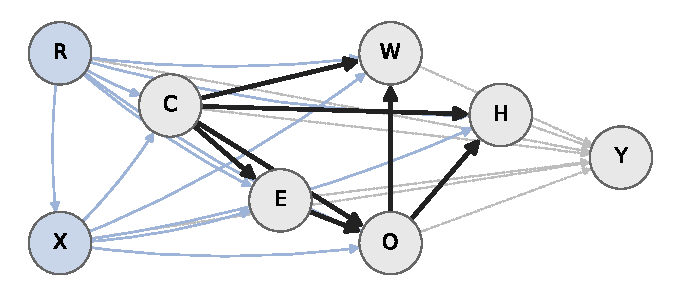
\includegraphics[width=\linewidth]{figures/bn_dag.pdf}\\
{\scriptsize Learned in all six domains. Blue: required $R,X$ edges.}
\end{column}
\begin{column}{0.48\textwidth}
\small
\begin{itemize}[<+->]
\item All 8 variables observed; the graph is associational.
\item Composition: $P(v\mid R,X,\mathrm{pa}'(v))$, Dirichlet-smoothed.
\item Outcome: log-linear $P(Y\mid \text{all features})$.
\item Query $P(G,\mathrm{pa}(Y),Y)$ gives each group's TPR and FPR.
\item VE $=$ clique tree $=$ enumeration $=$ pgmpy (error $1.3\times10^{-15}$).
\end{itemize}
\end{column}
\end{columns}
\end{frame}

% Slide 6: 60 seconds. Student 2 starts.
\begin{frame}{Fairness criterion and proposed method}
\begin{itemize}[<+->]
\item \textbf{Fairness:} $\EO = \max(\text{TPR gap}, \text{FPR gap})$ across groups. Errors should not depend on the
group, given the true label.
\item \textbf{Utility:} balanced accuracy; at most 0.02 loss allowed.
\item \textbf{BN-LFA} for each factor: Bayes factor of a shift $\times$ its exact effect on the fair rule, then update
the top $\le 2$ factors.
\item Refit thresholds on source data weighted by $w=\prod_{v\in F}\hat\theta_t/\theta_s$.
\item Uses race and sex at prediction time (features and group thresholds).
\end{itemize}
\end{frame}

% Slide 7: 60 seconds.
\begin{frame}{Experimental protocol}
\begin{itemize}[<+->]
\item \textbf{Baselines:} LR, GBT, reweighing, EO-S (keep source rule), TT (target thresholds), IW-EO, retraining,
BN-S, BN-all.
\item Every method gets the same $n$ target persons. Test labels are never used for fitting.
\item 9 transfers $\times$ 6 budgets $\times$ 5 seeds.
\item Paired household bootstrap ($B = 2000$); Holm over 6 confirmatory tests.
\item Plus a synthetic simulation, ablations and robustness tests.
\end{itemize}
\end{frame}

% Slide 8: 90 seconds.
\begin{frame}{Main result and uncertainty}
\begin{columns}[T]
\begin{column}{0.46\textwidth}
\small
\begin{tabular}{lcc}\toprule
Method, $n=1000$ & BA & $\EO$\\\midrule
EO-S (source rule) & 0.771 & 0.150\\
TT & 0.772 & 0.205\\
IW-EO (closest) & 0.769 & 0.156\\
BN-all & 0.770 & 0.147\\
\textbf{BN-LFA} & 0.770 & \textbf{0.140}\\\bottomrule
\end{tabular}\\[3pt]
{\scriptsize Mean of 9 transfers $\times$ 5 seeds; lower $\EO$ is fairer.}
\end{column}
\begin{column}{0.54\textwidth}
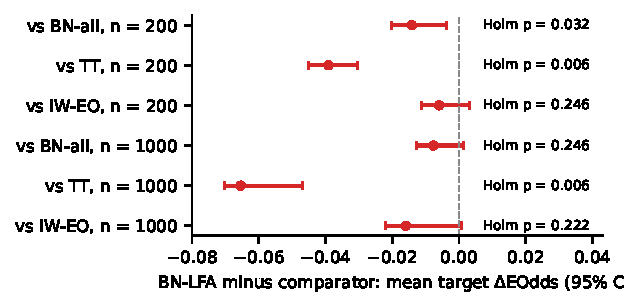
\includegraphics[width=\linewidth]{figures/confirmatory_forest.pdf}
\end{column}
\end{columns}
\vspace{6pt}
\textbf{Answer: partially supported.} BN-LFA is fairer than TT (both budgets) and BN-all ($n=200$), but not than
IW-EO or the unchanged source rule.
\end{frame}

% Slide 9: 60 seconds.
\begin{frame}{Ablation, robustness and failure case}
\small
\begin{itemize}[<+->]
\item \textbf{Ablation} ($n=1000$): random factors 0.152 and all factors 0.147, vs BN-LFA 0.140.
\item \textbf{Mechanism:} the diagnostic predicts the fairness change (Spearman 0.88).
\item \textbf{Failure:} three shifted factors but only two allowed: no better than EO-S (0.187 vs 0.184).
\end{itemize}
\begin{center}
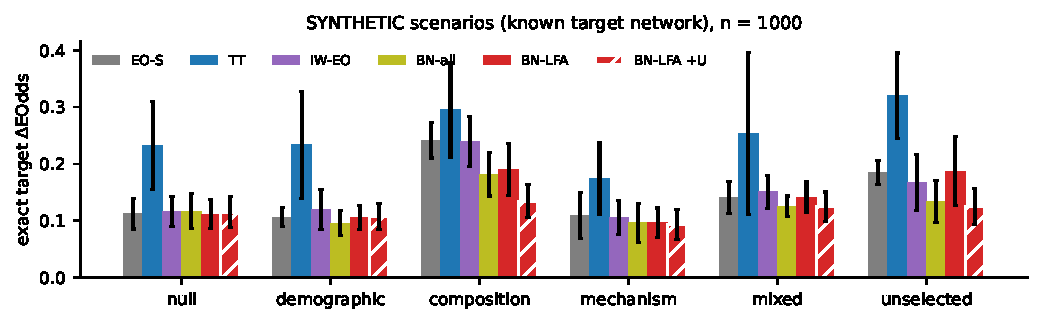
\includegraphics[width=0.74\linewidth]{figures/simulation.pdf}\\[-2pt]
{\scriptsize SYNTHETIC: with unlabelled data, BN-LFA fixes a group-specific shift that IW-EO cannot (0.134 vs 0.220).}
\end{center}
\end{frame}

% Slide 10: 60 seconds. Total suggested main talk: 10 minutes.
\begin{frame}{Conclusion and reproducibility}
\begin{itemize}[<+->]
\item \textbf{Conclusion:} with few labels, adapting $\le 2$ factors beats refitting thresholds, but gives no reliable
gain over reweighting or no adaptation.
\item \textbf{Limits:} associational graph; 3 states, 2 years; small groups; the \$50k label; race and sex used at
decision time.
\item \textbf{Reproduce:} \texttt{github.com/aslammugutkhan/fairness-transfer} (commit \texttt{2eaef71}): \emph{Run all} in the notebook on Colab (13 min).
\end{itemize}
\end{frame}

\appendix
\begin{frame}{Backup: mandatory evidence and references}
\small
\begin{tabular}{p{0.45\linewidth}p{0.42\linewidth}}\toprule
Requirement (Problem 5) & Evidence in \texttt{results/}\\\midrule
E1--E3: within-domain, transfers, budgets & \texttt{exp\_transfer\_summary.csv}, Figs.\ 2--3\\
E4: composition vs mechanism simulation & \texttt{sim\_all\_runs.csv}, Fig.\ 7\\
E5: method comparison & \texttt{confirmatory\_tests\_holm.csv}\\
Ablations; robustness tests & \texttt{ablation\_d\_eodds.csv}, \texttt{robustness\_summary.csv}\\\bottomrule
\end{tabular}\\[6pt]
\footnotesize Full matrix: \texttt{docs/requirements\_matrix.md}. Key references: Ding et al.\ 2021; Shao et al.\
2024; Hardt et al.\ 2016; Schrouff et al.\ 2022; Singh et al.\ 2021; Pearl \& Bareinboim 2011
(16 papers in \texttt{docs/related\_work.md}).
\end{frame}

\begin{frame}{Backup: inference and statistical validation}
\begin{itemize}
\item CPTs normalised; factor algebra, evidence and missing values checked (notebook self-checks).
\item 20 random queries: all exact methods agree to $1.3\times10^{-15}$. Elimination order changes cost only.
\item Every local Markov statement is a d-separation; largest residual dependence 0.047 bits.
\item Model-based group TPRs within sampling noise for 89\,\% of groups.
\item Bootstrap resamples households; the same resamples for all methods (paired).
\end{itemize}
\end{frame}

\begin{frame}{Backup: demonstration and individual defence}
\begin{itemize}
\item Run notebook section 2.12 (a few seconds).
\item $P(Y{=}1\mid\text{Black, female, graduate}) = 0.6636$ by VE, clique tree and enumeration.
\item CA18$\to$TX18 with 200 labels: BN-LFA updates $E$ and $R$; $\EO$ 0.143 vs 0.156 (EO-S), 0.237 (TT).
\item Why $R$ barely matters: equalized odds conditions on the group, so race mix alone does not move error rates.
\item Saved trace: \texttt{demo/demo\_trace.txt}.
\end{itemize}
\end{frame}
\end{document}
